%\section{\label{I-A-1}La représentation nationale : un musée aux collections uniques}
%
%\subsection{La lente construction du \mae}\footnote{Voir la chronologie de l'histoire du musée en Annexe \ref{Ax-A}.}
%
%L’histoire du \acf{mae} est celle d’un projet persistant, sans cesse reporté et modifié, qui trouve ses racines dans les aspirations d'associations ou de personnalités liées à l'aéronautique dès la fin du XIXe siècle\footcite{terrierAeroportParisBourget2019}. Aujourd'hui encore il ne cesser d'évoluer, et cette année 2025 aura vu, en plus de modernisations importantes de son environnement logiciel, l'inauguration d'un nouvel espace d'exposition permanente mettant en valeur la tour de contrôle de l'aéroport historique du Bourget\footcite{museedelairetdelespaceHallNavigationAerienne2025}. C'est en effet dans ces locaux que le musée s'est installé en 1973, après une longue période de recherches pour une installation définitive. Confronté aux évènements du XXe siècle, aux difficultés de conservation d'objets volumineux et techniques et aux aléas des tutelles ministérielles, c'est principalement grâce à l'impulsion de militaires, de passionnés d'aéronautique et à sa fonction de représentation d'un savoir faire technique français qu'il a pu voir le jour.
%
%La décision devient effective après la Première Guerre Mondiale, premier conflit armé à reconnaître l'importance stratégique de l'aviation. A l'initiative d'Albert Caquot, un conservatoire de l'aéronautique est confié au capitaine Hirschauer et quelques aéronefs trouvent refuge dans un hangar à Issy-les-Moulineaux avant qu'une crue de la Seine ne contraigne leur repli à Chalais-Meudon. Le musée est officiellement inauguré le 23 novembre 1921 : l’institution est née, mais son ancrage reste fragile.
%Pendant l’entre-deux-guerres, le musée s’essaie à d’autres implantations, notamment à Paris, boulevard Victor. Ces locaux sont inaugurés en 1936, mais fermés trois ans plus tard à l’aube de la Seconde Guerre Mondiale. Les bombardements puis la saisie allemande de collections en transit brisent son élan : à la Libération, le musée réintègre Chalais-Meudon, mais il reste fermé au public pendant plus de quinze ans.
%
%L’histoire qui suit est celle d’une errance administrative et territoriale. Vingt-et-un sites sont envisagés entre 1952 et 1972\footcite{terrierAeroportParisBourget2019} : Orly, Versailles, Issy-les-Moulineaux… Aucun ne fait l’unanimité. En 1961, le musée rouvre au public à Meudon, mais c’est une solution provisoire. Le « Palais de l’Air et de l’Espace » continue à chercher les locaux qui pourront mettre en valeur ses collections dans tout leur volume, et il faudra attendre 1973 pour que l'ancien aéroport du Bourget, dont l'activité vient d'être drastiquement réduite après l’essor d'Orly, soit retenu comme implantation définitive.
%
%Dès son ouverture au Bourget, le musée témoigne d'un lien privilégié avec l'industrie aéronautique française et l'état : pour son ouverture, le prototype du Concorde 001 lui est donné. Dès lors, les collections sont progressivement transférées depuis Chalais-Meudon qui ferme en 1981, la direction rejoint les locaux du Bourget, et de nouveaux halls sont inaugurés au fil de la mise à disposition et le rachat de nouveaux bâtiments libérés par l'aéroport. En 1983, à l'occasion de l'inauguration d'un nouveau hall consacré aux collections spatiales, le musée prend officiellement son nom actuel de \acf{mae}.
%
%Ce mouvement de consolidation du musée et d'intégration dans le réseau des musées techniques français se consolide à cette période, notamment avec l'ouverture du Planétarium (1985), la création de réserves et d'un atelier de restauration sur la commune de Dugny,  ou l'informatisation du musée. Dès la fin des années 1990 sont en effet mis en place Micromusée, logiciel de gestion des collections et le \ac{sigb} Alexandrie. Cette mise en place est suivie à partir de 2016 par la mise en ligne d'un logiciel exclusivement dédié à la gestion et la diffusion de fichiers audiovisuels : l'e-médiathèque du musée. Celui-ci devient une institution muséale à part entière qui se professionnalise petit à petit, le \mae est labellisé « Musée de France » depuis 2002.
%
%Aujourd’hui, l’établissement poursuit son développement en renouvelant ses outils bibliothéconomiques et muséaux, en inaugurant de nouveaux espaces de conservation et d'exposition, et son intégration prochaine au réseau du Grand Paris Express laisse espérer un accroissement de son attractivité auprès du public. L’histoire du \mae est ainsi celle d'un projet, qui s’est construit autour de ses collections et non à partir d’un site, entièrement dédié à la mémoire du ciel.
%
%\subsection{Une institution complexe qui fait référence}
%C’est donc à partir des années 1980 que le musée s’est véritablement construit et transformé, sous l’effet conjoint d’une reconnaissance de l’importance culturelle du secteur aéronautique, du renouvellement de la réflexion sur la muséologie et d’une volonté d'inscrire l'institution dans le réseau national des musées. Le déménagement du musée au Bourget est révélateur de la double fonction qu’il occupe aujourd’hui : à la fois conservatoire historique d’un patrimoine technique, et vitrine nationale d’une industrie stratégique. L’aéroport du Bourget, premier aérodrome civil de Paris\footcite{terrierAeroportParisBourget2019}, est en effet un lieu hautement symbolique qui inscrit le musée dans la géographie comme dans l'histoire de l'aviation française : cette localisation unique confère encore davantage de légitimité au musée. Son lien étroit avec le \ac{siae} qu'il accueille tous les deux ans assied également sa dimension promotionnelle, qui mêle l’histoire à la modernité, et la culture au dynamisme industriel.
%
%Par-delà son histoire et sa structure, ce qui distingue avant tout le Musée de l’Air et de l’Espace, c’est la richesse et la diversité de ses collections, qui en font une référence nationale sans équivalent. On y trouve, bien sûr, des avions historiques, des moteurs, des équipements techniques — objets dont la conservation requiert des conditions très spécifiques et une expertise rare. Cette particularité technique, sans précédent dans les musées français, impose une gestion adaptée et des vocabulaires spécialisés. Mais la collection ne se limite pas à ces objets spectaculaires. S’y ajoutent des maquettes, des estampes, des objets d’art, et des ensembles communs aux musées militaires, tels que des uniformes. La prise en compte, plus récente, des collections civiles — vêtements d’aviateurs civils, objets du quotidien — témoigne d’une évolution de la politique muséale vers une approche plus anthropologique, qui valorise l’histoire sociale et humaine de l’aéronautique. Cette évolution se manifeste principalement avec la création du [TODO: date de remaniement de l'organigramme] département des collections artistiques et anthropologiques\footnote{TODO: image thésaurus des domaines}, s'occupant de la gestion d'objets relevant de la représentation de l'aéronautique dans la société ou la culture : arts graphiques ou sculpture, mais encore objets du quotidien comme de la vaisselle ou des jouets\footcite{collectifMuseeLairLespace2023}.
%
%Cette singularité du musée reflète une réalité plus large, celle des musées techniques, qui occupent une place particulière dans le paysage muséal français. Confrontés à des réalités bien différentes des musées de beaux-arts, ces établissements rencontrent des difficultés spécifiques. Leurs chargés de collections doivent être formés à la fois aux savoirs techniques et aux pratiques muséales : on observe ainsi que les plus jeunes générations de chargés de collections du musée de l'air et de l'espace proviennent souvent de masters spécialisés dans des musées techniques -- le master Muséologie des Sciences de la Nature et de l'Homme au museum d'histoire naturelle par exemple -- et gravitent entre des institutions comme les différents musées de l'armée -- musée de la marine, musée de l'armée aux Invalides -- et d'autres musées techniques comme le \ac{cnam}. Ces musées doivent sans cesse composer avec la nature même de leurs collections — des objets souvent volumineux, dont les matériaux peuvent avoir des exigences de conservation très particulières, souvent uniques au musée — ce qui impose des méthodes innovantes et une adaptation constante. Cette problématique est parfaitement résumée par Agnès Mirambet-Paris et François Mirambet dans un article sur la conservation et restauration du patrimoine : les principales difficultés identifiées sont notamment la complexité des matériaux conservés, leur état de dégradation avancé, des environnements de conservation souvent peu adaptés, les problèmes posés par l'échelle des objets concernés, les ressources importantes que cela nécessite et la lourdeur de procédures administrative et des financements que  nécessite la conservation de tels objets\footcite{mirambet-parisConservationrestaurationPatrimoineTechnique2011}. Les deux professionnels du patrimoine concluent en insistant sur le fait que 
%\begin{quote}
%	\og C’est bien par le partage de compétences techniques acquises dans le domaine industriel et celles obtenues dans les écoles de formation à la restauration que pourront se développer pleinement des travaux de restauration\footcite{mirambet-parisConservationrestaurationPatrimoineTechnique2011}.\fg
%\end{quote}
%
%Ainsi, le Musée de l’Air et de l’Espace s’inscrit dans cette catégorie d’institutions où l’expertise technique se mêle à l’exigence muséale, et le caractère exceptionnel de ses collections -- certains modèles, comme le prototype du Concorde 001 ou le scaphandre de Jean-Loup Chrétien, sont en effet uniques au monde\footcite{champenoisTresorsMuseeLair}. Cette position, fragile et exigeante, le place au carrefour des enjeux de représentation nationale, de conservation patrimoniale, et d’innovation culturelle.

\section{\label{I-A-1}La représentation nationale : un musée aux collections uniques}

\subsection{La lente construction du \mae}

L’histoire du \acf{mae}\footnote{Voir la chronologie de l'histoire du musée en Annexe \ref{Ax-A}.} est celle d’un projet persistant, sans cesse reporté et modifié, qui trouve ses racines dans les aspirations d'associations ou de personnalités liées à l'aéronautique dès la fin du XIXe siècle\footcite{terrierAeroportParisBourget2019}. Aujourd'hui encore, il ne cesse d'évoluer : l’année 2025 aura vu, outre des modernisations logicielles majeures, l'inauguration d’un nouvel espace d’exposition permanente valorisant la tour de contrôle de l’aéroport historique du Bourget\footcite{museedelairetdelespaceHallNavigationAerienne2025}. C’est dans ces locaux que le musée s’est installé en 1973, après une longue période de recherches pour une implantation pérenne. Confronté aux aléas du XXe siècle, aux contraintes de conservation d’objets techniques et aux hésitations ministérielles, il doit sa concrétisation à l’engagement de militaires, de passionnés et à sa vocation de vitrine d’un savoir-faire français.

La décision devient effective après la Première Guerre mondiale, premier conflit à reconnaître l’importance stratégique de l’aviation. À l’initiative d’Albert Caquot, un conservatoire de l’aéronautique est confié au capitaine Hirschauer : quelques aéronefs trouvent refuge à Issy-les-Moulineaux, avant d’être déplacés à Chalais-Meudon à la suite d’une crue de la Seine. Le musée est officiellement inauguré le 23 novembre 1921 : l’institution naît, mais sans réel ancrage.

Pendant l’entre-deux-guerres, il tente d’autres implantations, notamment boulevard Victor à Paris. Ces locaux, ouverts en 1936, ferment trois ans plus tard à l’aube de la Seconde Guerre mondiale. Bombardements et saisies allemandes interrompent son élan ; à la Libération, le musée réintègre Chalais-Meudon, mais reste fermé au public durant plus de quinze ans.

Suit une errance institutionnelle et territoriale : vingt-et-un sites sont envisagés entre 1952 et 1972\footcite{terrierAeroportParisBourget2019}. En 1961, le musée rouvre à Meudon, mais provisoirement. Le « Palais de l’Air et de l’Espace » poursuit sa quête de locaux adaptés à la monumentalité de ses collections. En 1973, l’ancien aéroport du Bourget, libéré au profit d’Orly, est retenu comme implantation définitive.

Dès son ouverture, le musée affirme un lien fort avec l’État et l’industrie aéronautique : le Concorde 001 lui est offert. Les collections sont progressivement transférées, Chalais-Meudon ferme en 1981, la direction rejoint le Bourget, de nouveaux halls sont ouverts au fil de l’extension du site. En 1983, à l’occasion d’un nouveau hall spatial, le musée prend son nom actuel : \acf{mae}.

Cette consolidation s’accompagne de son intégration au réseau des musées techniques : ouverture du Planétarium (1985), création de réserves à Dugny, informatisation. Fin des années 1990 : mise en place de Micromusée pour les collections, et du \ac{sigb} Alexandrie pour la bibliothèque. En 2016, l’e-médiathèque est lancée pour les fonds audiovisuels. Le \mae, labellisé « Musée de France » depuis 2002, se professionnalise.

Aujourd’hui, il poursuit sa modernisation : renouvellement des outils de gestion, nouveaux espaces de conservation et d’exposition. Son intégration au réseau du Grand Paris Express laisse espérer un surcroît de fréquentation. Le \mae est ainsi un musée né de ses collections, et non d’un site, dédié à la mémoire du ciel.

\subsection{Une institution complexe qui fait référence}

C’est à partir des années 1980 que le musée se structure véritablement, sous l’effet conjoint d’une reconnaissance de l’importance culturelle de l’aéronautique, d’un renouveau muséographique et de son inscription dans les réseaux nationaux. Son installation au Bourget incarne sa double fonction : conservatoire historique et vitrine stratégique. Premier aérodrome civil parisien\footcite{terrierAeroportParisBourget2019}, ce lieu symbolique ancre le musée dans la géographie et l’histoire de l’aviation française. Son lien avec le \ac{siae}, qu’il accueille tous les deux ans, renforce sa fonction promotionnelle, entre tradition et innovation.

Ce qui distingue avant tout le Musée de l’Air et de l’Espace, c’est la richesse et l’hétérogénéité de ses collections, sans équivalent national. On y trouve des aéronefs, moteurs, équipements techniques — objets exigeant des conditions de conservation particulières et une expertise rare. Cette spécificité impose des pratiques adaptées et des vocabulaires spécialisés. Mais le musée ne s’y limite pas : maquettes, estampes, objets d’art, uniformes, et, plus récemment, objets civils — vêtements, vaisselle, jouets — reflètent une évolution vers une muséographie anthropologique. Cette inflexion est incarnée notamment par la création d'un département des collections artistiques et anthropologiques, et la diversité des objets conservés se retrouve dans le schéma ci-dessous qui rassemble les différents noms de domaines des collections du musée.

\begin{figure}[htbp]
	\centering
	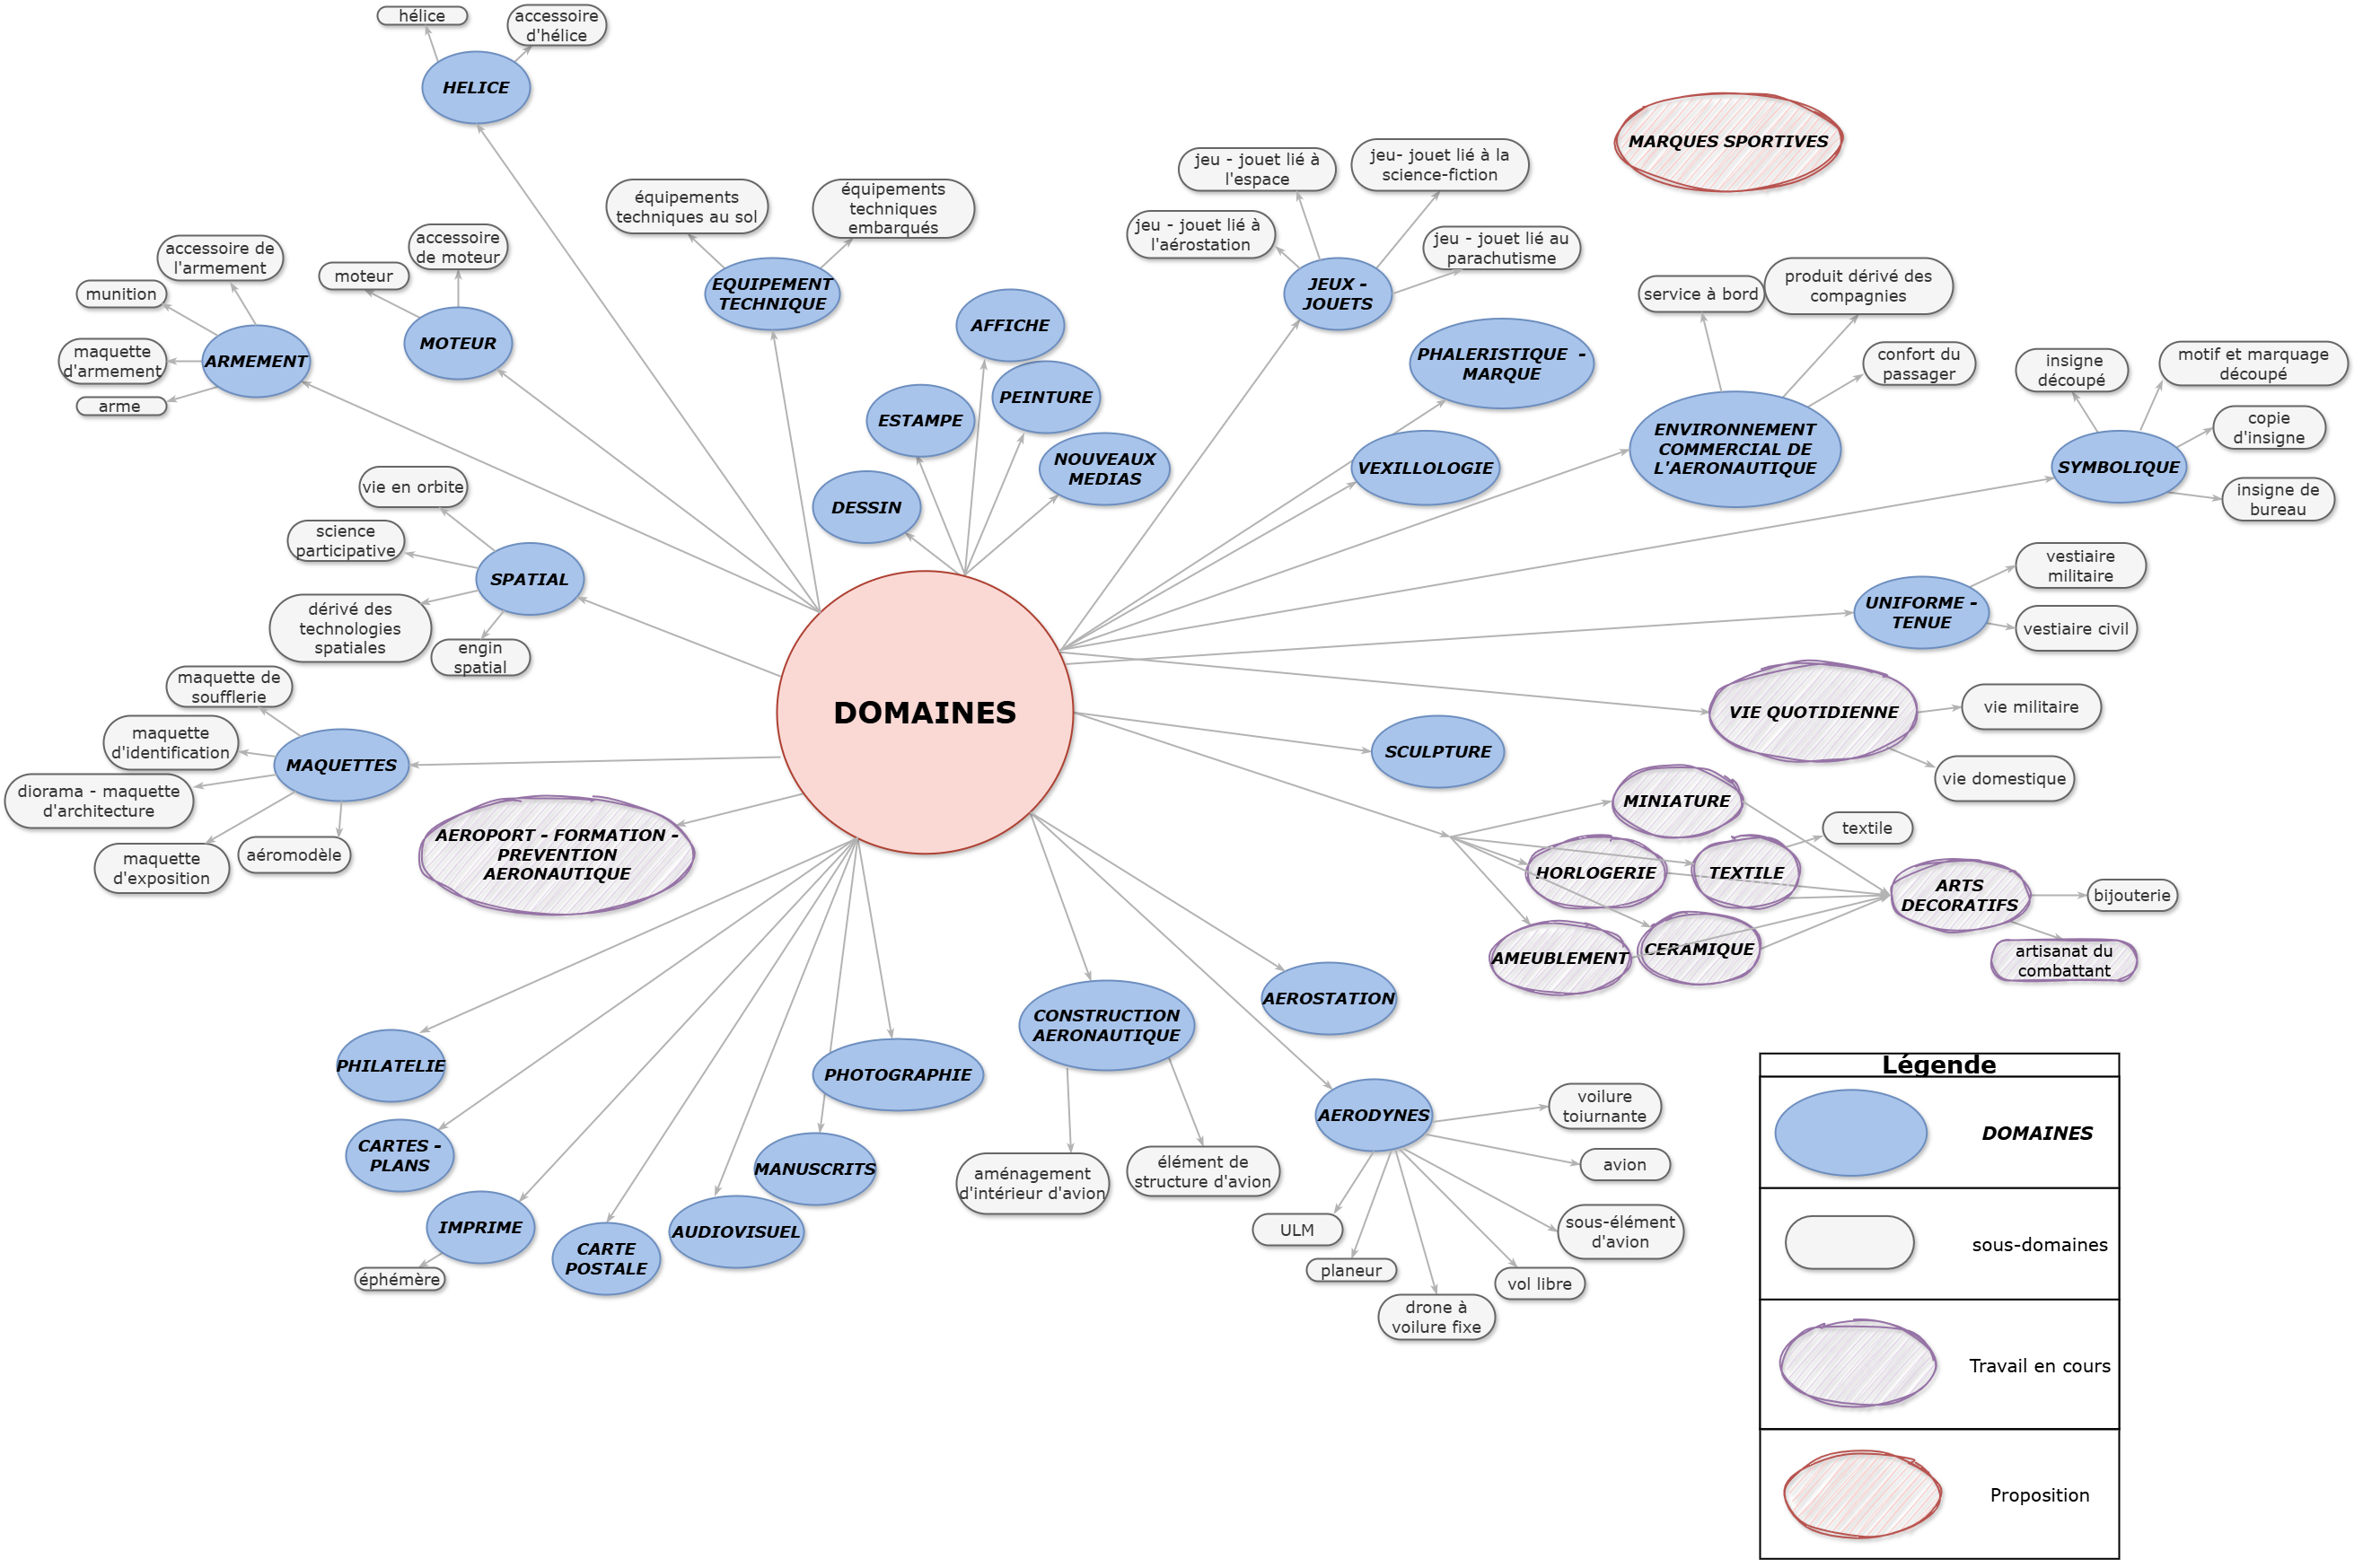
\includegraphics[width=\linewidth]{img/MODEL_domaines.png}
	\caption{Modélisation du thésaurus des domaines utilisés par le \mae}
	\label{fig:model_domaines}
\end{figure}

Le \mae incarne donc des défis propres aux musées techniques, bien différents de ceux des musées de beaux-arts et qui imposent des compétences croisées à la fois techniques et muséales. Les jeunes chargés de collections sont ainsi souvent issus de formations spécialisés — comme les masters du Muséum d’histoire naturelle — et passent par des institutions techniques ou militaires, telles que le musée de la Marine, le musée de l’Armée ou le \ac{cnam}. Ces musées doivent sans cesse composer avec des objets singuliers, souvent massifs, complexes à restaurer et à exposer.

Ces multiples défis sont rappelés par Agnès Mirambet-Paris et François Mirambet : diversité des matériaux, état de dégradation, inadéquation des environnements de conservation, échelle des objets, lourdeur des procédures, et besoin de ressources spécialisées\footcite{mirambet-parisConservationrestaurationPatrimoineTechnique2011}. Ils insistent sur la nécessité du dialogue entre techniciens et restaurateurs :
\begin{quote}
	\og C’est bien par le partage de compétences techniques acquises dans le domaine industriel et celles obtenues dans les écoles de formation à la restauration que pourront se développer pleinement des travaux de restauration\footcite{mirambet-parisConservationrestaurationPatrimoineTechnique2011}.\fg
\end{quote}

Le \mae incarne cette articulation entre expertise technique et exigence muséale. Ses pièces emblématiques — comme le Concorde 001 ou le scaphandre de Jean-Loup Chrétien\footcite{champenoisTresorsMuseeLair} — en font une institution unique, au croisement des enjeux de représentation nationale, de préservation patrimoniale et d’innovation culturelle.
